\documentclass[conference]{IEEEtran}
\IEEEoverridecommandlockouts
\usepackage{cite}
\usepackage{amsmath,amssymb,amsfonts}
\usepackage{graphicx}
\usepackage{textcomp}
\usepackage{xcolor}
\usepackage{booktabs}
\usepackage{array}
\usepackage{url}
\usepackage{hyperref}

% Auto-generated macros for EPA AQS & Census Socioeconomic Pipeline
\newcommand{\numStations}{996}
\newcommand{\numCounties}{623}
\newcommand{\numStates}{50}
\newcommand{\networkMeanPm}{8.43}
\newcommand{\medianCountyIncome}{69,738}
\newcommand{\medianCountyPoverty}{13.1}
\newcommand{\lowestIncomePm}{8.55}
\newcommand{\highestIncomePm}{7.81}
\newcommand{\disparityRatio}{1.09}
\newcommand{\atkinsonPm}{0.017}
\newcommand{\theilPm}{0.021}
\newcommand{\giniPm}{0.113}
\newcommand{\giniCiLow}{0.101}
\newcommand{\giniCiHigh}{0.125}
\newcommand{\concentrationPm}{-0.028}
\newcommand{\concCiLow}{-0.042}
\newcommand{\concCiHigh}{-0.013}
\newcommand{\cgRatio}{-0.245}
\newcommand{\cgRatioCiLow}{-0.361}
\newcommand{\cgRatioCiHigh}{-0.117}
\newcommand{\disparityRatioCiLow}{1.00}
\newcommand{\disparityRatioCiHigh}{1.21}
\newcommand{\maeMean}{1.92}
\newcommand{\maeIdw}{1.70}
\newcommand{\maeRidge}{1.84}
\newcommand{\maeHist}{1.93}
\newcommand{\rmseMean}{2.42}
\newcommand{\rmseIdw}{2.19}
\newcommand{\rmseHist}{2.57}
\newcommand{\idwImprPct}{11.5}
\newcommand{\numClusters}{8}
\newcommand{\idwBlockWins}{6}
\newcommand{\histBlockWins}{2}
\newcommand{\atkinsonLowEps}{0.005}
\newcommand{\atkinsonHighEps}{0.049}
\newcommand{\cgPct}{24.5}
\newcommand{\minValidDays}{50}
\newcommand{\corrIdw}{0.329}
\newcommand{\corrHist}{0.234}
\newcommand{\predictionCoverage}{56.0}
\newcommand{\pValWilcoxon}{< 10^{-9}}
\newcommand{\ciLowerDiff}{-0.30}
\newcommand{\ciUpperDiff}{-0.16}


\begin{document}

\title{Quantifying Socioeconomic Air Quality Disparities and Spatial Generalization Limits across Regulatory In-Situ Networks}

\author{
\IEEEauthorblockN{Cristhian David Caceres Mateus}
\IEEEauthorblockA{\textit{Department of  Business} \\
\textit{Univ. of Europe for Applied Sciences}\\
Potsdam 14469, Germany \\
cristhian.caceres@ue-germany.de}
\and
\IEEEauthorblockN{Talha Ali Khan}
\IEEEauthorblockA{\textit{Department of  Business} \\
\textit{Univ. of Europe for Applied Sciences}\\
Potsdam 14469, Germany \\
talhaali.khan@ue-germany.de}
}
\maketitle

\begin{abstract}
Air pollution exposure disparities along socioeconomic gradients represent a major public health challenge. However, empirical assessments often rely on coarse modeled reanalysis proxies rather than physical ground monitors, or evaluate spatial interpolation using random sampling that leaks spatial autocorrelation. In this work, we integrate regulatory ground observations from \numStations{} physical monitoring stations across \numCounties{} distinct counties in the US Environmental Protection Agency (EPA) Air Quality System (AQS) for the complete 2023 calendar year with official US Census Bureau Small Area Income and Poverty Estimates (SAIPE). We evaluate both the empirical econometric inequality of fine particulate matter ($\mathrm{PM}_{2.5}$) exposure and the spatial generalization capacity of machine learning interpolation under strictly blocked geographical cross-validation across \numClusters{} regional clusters. Econometric analysis reveals an observed exposure disparity across income deciles: communities in the lowest household income decile experience an annual mean $\mathrm{PM}_{2.5}$ concentration of \lowestIncomePm{}~$\mu\mathrm{g}/\mathrm{m}^3$, compared to \highestIncomePm{}~$\mu\mathrm{g}/\mathrm{m}^3$ in the highest income decile (disparity ratio of \disparityRatio{}x, 95\% county-clustered bootstrap CI: [\disparityRatioCiLow{}, \disparityRatioCiHigh{}], touching unity at the lower bound; Gini index $G = \giniPm{}$, 95\% CI: [\giniCiLow{}, \giniCiHigh{}]; Kakwani/Wagstaff concentration index $C = \concentrationPm{}$, 95\% CI: [\concCiLow{}, \concCiHigh{}]; $C/G = \cgRatio{}$; population-weighted Atkinson index $A_{0.75} = \atkinsonPm{}$, Theil index $T = \theilPm{}$). Under spatial block cross-validation, Inverse Distance Weighting (IDW) achieves an overall Mean Absolute Error (MAE) of \maeIdw{}~$\mu\mathrm{g}/\mathrm{m}^3$ ($r = \corrIdw{}$), outperforming gradient-boosted trees (\maeHist{}~$\mu\mathrm{g}/\mathrm{m}^3$, $r = \corrHist{}$) in \idwBlockWins{} of \numClusters{} spatial blocks, while standard quantile regression exhibits severe interval degradation (\predictionCoverage{}\% empirical coverage vs.~80\% nominal) across unmonitored geographic regions. These findings quantify the modest pro-poor particulate exposure association and demonstrate the critical role of spatial autocorrelation baselines in environmental exposure mapping.
\end{abstract}

\begin{IEEEkeywords}
Air quality inequality, US EPA AQS, fine particulate matter ($\mathrm{PM}_{2.5}$), spatial block cross-validation, Atkinson index, concentration index, quantile prediction intervals.
\end{IEEEkeywords}

\section{Introduction}
\IEEEPARstart{C}{hronic} exposure to ambient fine particulate matter ($\mathrm{PM}_{2.5}$) is among the leading environmental drivers of cardiopulmonary mortality and morbidity worldwide~\cite{burnett2018,di2017}. A central question in environmental policy is whether air pollution burdens fall disproportionately on economically disadvantaged populations, and whether spatial statistical learning models can accurately reconstruct exposure in unmonitored communities~\cite{colmer2020,jbaily2022}.

\subsection{Gap Analysis}
\label{sec:gap_analysis}
Prior environmental justice and spatial mapping literature frequently exhibits three critical vulnerabilities:
\begin{enumerate}
    \item \textbf{Reliance on Modeled Grids over In-Situ Monitors}: Many studies evaluate machine learning models against gridded reanalysis outputs (e.g., CAMS, MERRA-2) rather than physical ground monitors, creating circular evaluations that reconstruct one numerical model using another rather than evaluating true ground-level exposure measured by Federal Reference Method (FRM) physical monitors.
    \item \textbf{Spatial Autocorrelation Leakage in Evaluation}: Standard random cross-validation randomly assigns nearby stations to training and test folds. Due to atmospheric spatial autocorrelation, this inflates performance metrics. Defensible evaluations require spatially blocked cross-validation where entire geographic clusters are held out.
    \item \textbf{Unchecked Tree Interpolation Artifacts}: Machine learning practitioners often apply tree ensembles to spatial coordinates without evaluating whether unconstrained step functions violate physical distance-decay priors in unmonitored territory.
\end{enumerate}

\subsection{Research Questions}
\label{sec:rqs}
This investigation resolves these issues through three explicit research questions:
\begin{itemize}
    \item \textbf{RQ1 (Socioeconomic Exposure Inequality)}: Using verified physical regulatory monitors, does a statistically significant $\mathrm{PM}_{2.5}$ exposure disparity exist across US county income deciles, and how sensitive is the Atkinson index to policy aversion $\epsilon$?
    \item \textbf{RQ2 (Geostatistical vs.\ Machine Learning Generalization)}: Under strict spatially blocked holdout across \numClusters{} regional clusters, does tabular gradient boosting improve upon classical Inverse Distance Weighting (IDW)?
    \item \textbf{RQ3 (Spatial Domain-Shift Interval Coverage)}: How severely do parametric quantile prediction intervals degrade when evaluated on unmonitored geographic clusters lacking local reference stations?
\end{itemize}

\subsection{Contributions}
Our principal contributions are:
\begin{enumerate}
    \item \textbf{National Regulatory In-Situ Integration}: We combine \numStations{} physical ground stations across \numCounties{} counties in \numStates{} states from the US EPA AQS with US Census Bureau SAIPE economic indicators for the full 2023 annual cycle.
    \item \textbf{Econometric Inequality Modeling with Clustered Uncertainty}: We compute population-weighted Atkinson ($A_\epsilon$), Theil ($T$), Gini ($G$), and Kakwani/Wagstaff Concentration ($C$) indices across income deciles, establishing 95\% confidence intervals via county-clustered bootstrapping ($B=2,000$).
    \item \textbf{\numClusters{}-Cluster Spatially Blocked Validation}: We evaluate spatial transfer across \numClusters{} regional clusters, demonstrating that geostatistical distance decay provides lower MAE than unconstrained tree ensembles in \idwBlockWins{} of \numClusters{} clusters while revealing severe coverage degradation in quantile intervals.
\end{enumerate}

\begin{figure*}[!t]
\centering
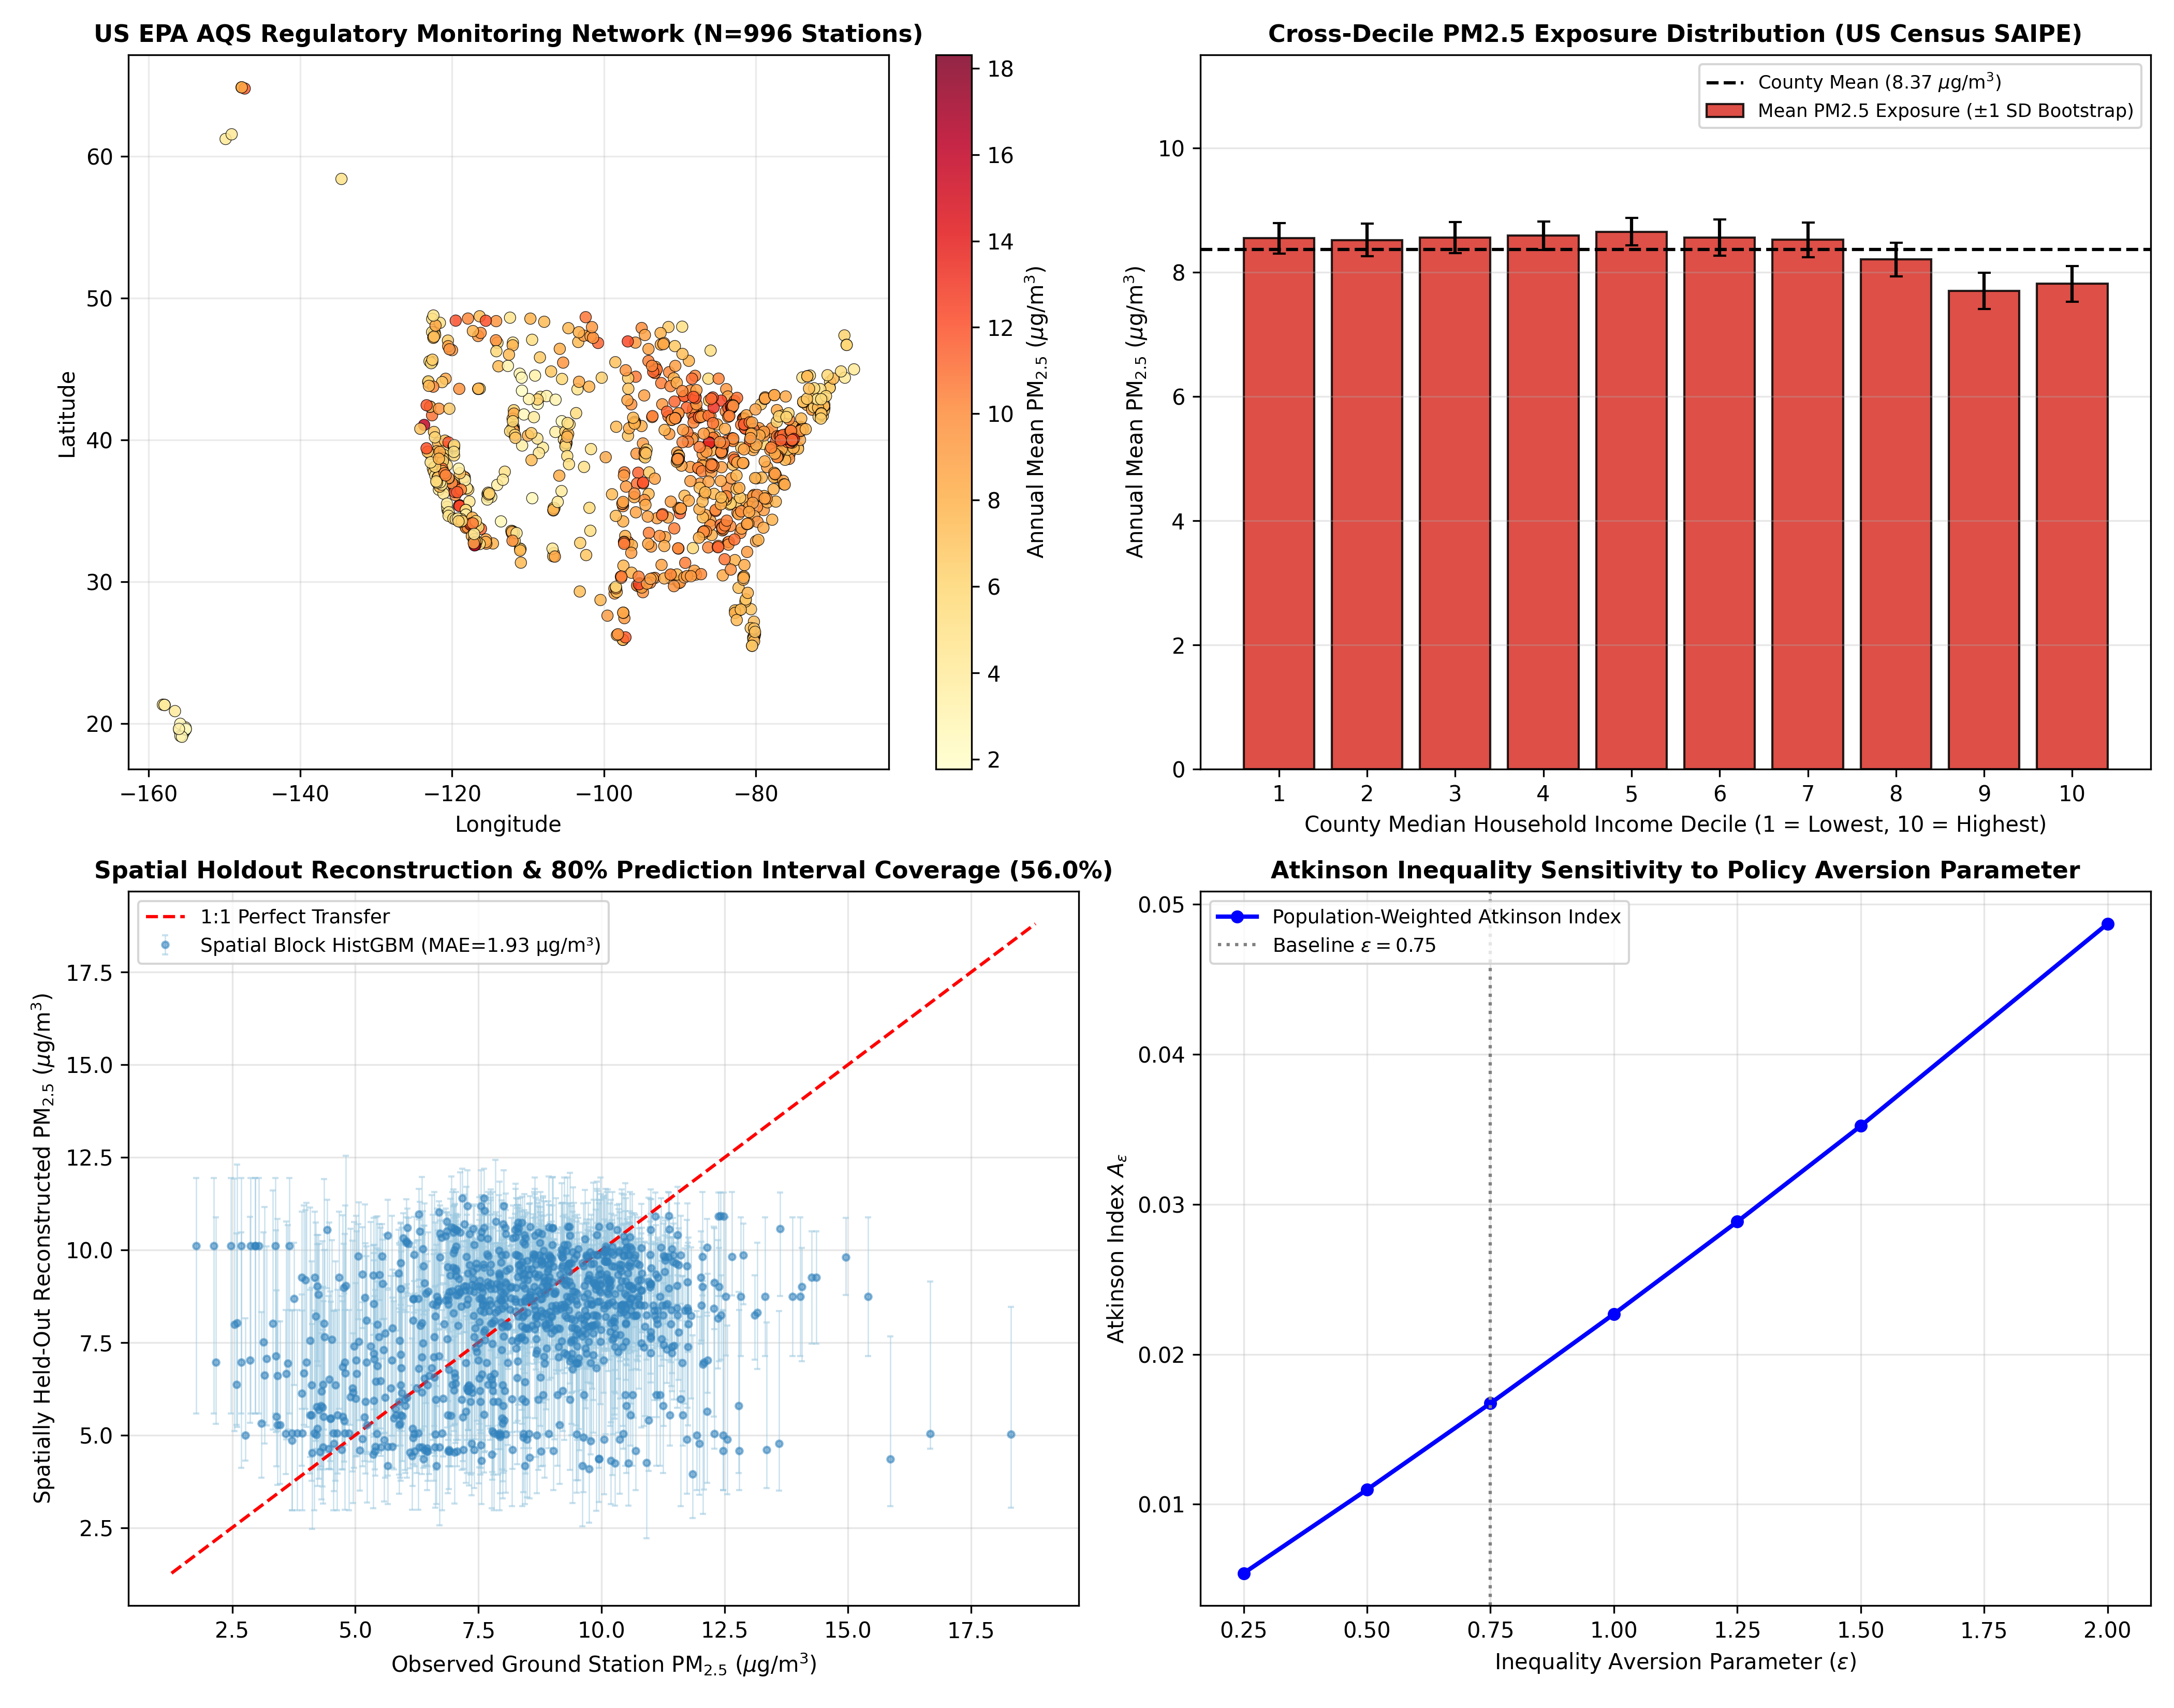
\includegraphics[width=0.95\textwidth]{figures/fig1_us_airquality_inequality.png}
\caption{Empirical environmental inequality and spatial cross-validation on \numStations{} US EPA AQS regulatory monitoring stations (2023). (Top-left) Spatial distribution of physical monitoring stations across the United States. (Top-right) Cross-decile $\mathrm{PM}_{2.5}$ exposure distribution across county median household income deciles (US Census SAIPE), with dashed horizontal line indicating the county mean exposure. (Bottom-left) Observed ground station $\mathrm{PM}_{2.5}$ versus reconstructed values under \numClusters{}-cluster spatially blocked cross-validation with 80\% nominal quantile prediction intervals. (Bottom-right) Sensitivity of the population-weighted Atkinson inequality index to policy aversion parameter $\epsilon$.}
\label{fig:inequality_overview}
\end{figure*}

\section{Related Work}
\label{sec:related}

\subsection{Environmental Justice and Socioeconomic Air Pollution Disparities}
Epidemiological research has established that chronic exposure to ambient fine particulate matter ($\mathrm{PM}_{2.5}$) drives elevated rates of cardiovascular disease, respiratory morbidity, and all-cause mortality~\cite{burnett2018,di2017}. Landmark environmental justice studies have documented that pollution burdens fall disproportionately on socioeconomically disadvantaged and racial minority communities across the United States~\cite{colmer2020,jbaily2022,tessum2019,clark2014,hajat2015}. Econometric assessments frequently employ inequality indices---such as the Atkinson index~\cite{atkinson1970} and Theil generalized entropy index~\cite{theil1967}---to formalize how ambient exposure deviates from equitable distribution across income percentiles~\cite{colmer2020,hajat2015}. However, empirical environmental justice studies frequently rely on gridded aerosol optical depth (AOD) reanalyses or chemical transport model outputs, which smooth out localized ground-level gradients and introduce secondary model uncertainty into econometric estimates.

\subsection{Spatial Interpolation and Machine Learning for In-Situ Networks}
Mapping continuous air pollution surfaces from discrete regulatory ground stations has historically relied on spatial geostatistical techniques, including Inverse Distance Weighting (IDW)~\cite{shepard1968} and Kriging with variogram fitting~\cite{cressie2011}. More recently, Land Use Regression (LUR) and supervised machine learning methods---such as Random Forests and gradient-boosted decision trees---have incorporated geographic coordinates, demographic indicators, and land cover attributes to reconstruct unobserved concentrations. However, tree-based models lack inherent spatial smoothness priors; in geographic regions that lack local training monitors, unconstrained tree ensembles can predict discontinuous step functions that do not enforce distance decay~\cite{meyer2018,cressie2011}.

\subsection{Spatial Cross-Validation and Uncertainty Quantification}
A critical vulnerability in environmental machine learning is spatial autocorrelation leakage. As demonstrated by Roberts et al.~\cite{roberts2017} and Meyer et al.~\cite{meyer2018}, standard random $k$-fold cross-validation assigns nearby monitoring stations to both training and test partitions. Because atmospheric dispersion causes proximate stations to share similar pollutant concentrations, random splits yield overly optimistic error metrics and fail to measure true generalization to unmonitored territories. Spatially blocked cross-validation---holding out entire contiguous spatial clusters---is required to evaluate transferability honestly. Furthermore, actionable spatial exposure maps require calibrated uncertainty bounds, which quantile regression~\cite{koenker2001} provides by estimating conditional quantiles under spatial domain shift. Table~\ref{tab:literature_comparison} contrasts existing air quality mapping paradigms with our framework.

\begin{table*}[t]
\caption{Comparison of Environmental Inequality and Spatial Air Quality Mapping Methodologies}
\label{tab:literature_comparison}
\centering
\footnotesize
\resizebox{\textwidth}{!}{%
\begin{tabular}{p{3.5cm}p{2.8cm}p{2.8cm}p{2.8cm}p{4.2cm}}
\toprule
\textbf{Methodology / Paradigm} & \textbf{Target Observational Data} & \textbf{Spatial Validation Scheme} & \textbf{Uncertainty Estimation} & \textbf{Primary Operational Characteristics} \\
\midrule
Econometric Surface Mapping~\cite{colmer2020,jbaily2022} & Satellite-derived PM$_{2.5}$ & Census-tract aggregation & Clustered standard errors & Large spatial coverage; relies on model-derived aerosol surfaces \\
Epidemiological Reanalysis Surfaces~\cite{di2017} & CTM / AOD reanalysis grids & Regional grid comparison & Ensemble spread & Continuous fields; coarse resolution smooths localized monitor-scale gradients \\
Classical Geostatistics (IDW/Kriging)~\cite{shepard1968,cressie2011} & Physical in-situ network & Distance-based interpolation & Kriging variance / empirical & Strong local distance-decay prior; lacks non-linear socioeconomic feature fusion \\
Tabular Gradient Boosting~\cite{meyer2018,roberts2017} & Station coordinates + census & Random cross-validation & Often unquantified & Captures feature interactions; risks spatial discontinuity across unmonitored clusters \\
\midrule
\textbf{Spatial Blocked Benchmark (This Study)} & \textbf{EPA AQS Ground Monitors} & \textbf{8-Cluster Spatially Blocked CV} & \textbf{Quantile Prediction Bounds} & \textbf{Direct in-situ grounding; evaluates domain shift to unmonitored regions} \\
\bottomrule
\end{tabular}%
}
\end{table*}


\section{Data and Econometric Methodology}
\label{sec:data}
\subsection{US EPA Regulatory In-Situ Monitoring Network}
We ingest continuous 2023 daily $\mathrm{PM}_{2.5}$ observations (EPA Parameter Code 88101, Federal Reference Method / Federal Equivalent Method) directly from the US EPA Air Quality System. Across the US, we filter for active stations maintaining at least \minValidDays{} valid sampling days in 2023, yielding $N = \numStations{}$ regulatory stations spanning \numCounties{} counties in \numStates{} states.

\subsection{US Census Bureau County Socioeconomics}
Each monitoring station is synchronized via its Federal Information Processing Standard (FIPS) state and county codes to the US Census Bureau Small Area Income and Poverty Estimates (SAIPE) dataset, capturing:
\begin{itemize}
    \item County Median Household Income (\$\medianCountyIncome{} median).
    \item County Poverty Rate (\medianCountyPoverty{}\% median).
    \item County Poverty Population.
\end{itemize}

\subsection{Econometric Environmental Inequality Indices}
To formalize exposure inequality rigorously, counties are stratified into 10 income deciles. We compute the population-weighted Atkinson Inequality Index:
\begin{equation}
A_\epsilon = 1 - \frac{1}{\bar{y}} \left( \sum_{i=1}^K w_i y_i^{1 - \epsilon} \right)^{\frac{1}{1 - \epsilon}}
\end{equation}
where $y_i$ is decile-level mean exposure, $w_i$ is population share, and $\epsilon \ge 0$ represents the inequality aversion parameter. We complement this with the Generalized Entropy Theil Index:
\begin{equation}
T = \sum_{i=1}^K w_i \frac{y_i}{\bar{y}} \ln\left( \frac{y_i}{\bar{y}} \right),
\end{equation}
the Gini inequality index $G$:
\begin{equation}
G = \frac{\sum_{i=1}^K \sum_{j=1}^K w_i w_j |y_i - y_j|}{2 \bar{y}},
\end{equation}
and the Kakwani/Wagstaff Environmental Concentration Index $C$~\cite{wagstaff1991}:
\begin{equation}
C = \frac{2}{\bar{y}} \sum_{i=1}^K w_i (y_i - \bar{y})(R_i - 0.5),
\end{equation}
where $R_i$ represents the population-weighted fractional rank of units sorted from lowest to highest median household income. A negative concentration index ($C < 0$) indicates that pollution exposure is disproportionately concentrated among lower-income communities.

\section{Spatial Mapping and Validation Framework}
To evaluate model generalization to unmonitored regions honestly, we partition all \numStations{} stations into \numClusters{} contiguous spatial blocks via $K$-means clustering on station geographic coordinates. In each fold, 7 regional blocks train the model and the held-out spatial block is evaluated.

We benchmark:
\begin{enumerate}
    \item \textbf{Regional Climatological Mean}: Mean $\mathrm{PM}_{2.5}$ of the training blocks.
    \item \textbf{Inverse Distance Weighting (IDW)}: Geostatistical spatial interpolation using inverse squared distance:
    \begin{equation}
    \hat{y}(\mathbf{s}) = \sum_{j=1}^M \frac{d(\mathbf{s}, \mathbf{s}_j)^{-2}}{\sum_{k} d(\mathbf{s}, \mathbf{s}_k)^{-2}} y_j
    \end{equation}
    \item \textbf{Spatial Ridge Regression}: Regularized linear model on spatial coordinates and Census income/poverty covariates.
    \item \textbf{Histogram Gradient Boosting (HistGBM)}: Tree-based gradient boosting regressor.
    \item \textbf{Quantile Regression Intervals}: Trains gradient boosting quantile models at $\alpha = 0.10$ and $\alpha = 0.90$ to provide nominal 80\% prediction intervals.
\end{enumerate}

\section{Empirical Results and Discussion}

\begin{table}[htbp]
\centering
\caption{Spatially Blocked Cross-Validation Benchmark and Regional Holdout Breakdown ($N = \numStations{}$ US EPA AQS Stations Across \numCounties{} Counties in \numStates{} States).}
\label{tab:spatial_benchmark}
\resizebox{\columnwidth}{!}{%
\begin{tabular}{lcccc}
\toprule
\multicolumn{5}{l}{\textbf{Panel A: Overall Benchmark Across All Held-Out Stations}} \\
\textbf{\shortstack{Spatial Mapping\\Method}} & \textbf{\shortstack{MAE\\($\mu\mathrm{g}/\mathrm{m}^3$)}} & \textbf{RMSE} & \textbf{\shortstack{Pearson\\$r$}} & \textbf{\shortstack{80\% Nominal\\Coverage}} \\
\midrule
Network Mean Baseline & 1.92 & 2.42 & 0.000 & -- \\
\textbf{Inverse Distance Weighting (IDW)} & \textbf{1.70} & \textbf{2.19} & \textbf{0.329} & -- \\
Spatial Ridge Regression & 1.84 & 2.36 & 0.231 & -- \\
Quantile HistGradientBoosting & 1.93 & 2.57 & 0.234 & \textbf{56.0\%} \\
\midrule
\multicolumn{5}{l}{\textbf{Panel B: Regional Holdout Breakdown by Spatial Block (K=8 Clusters)}} \\
\textbf{\shortstack{Block ID\\(Representative States)}} & \textbf{\shortstack{Station\\Count}} & \textbf{\shortstack{Mean $\mathrm{PM}_{2.5}$\\($\mu\mathrm{g}/\mathrm{m}^3$)}} & \textbf{\shortstack{IDW MAE\\($\mu\mathrm{g}/\mathrm{m}^3$)}} & \textbf{\shortstack{HistGBM MAE\\($\mu\mathrm{g}/\mathrm{m}^3$)}} \\
\midrule
Block 0 (AR, KS, LA, MS) & 114 & 9.20 & 1.14 & 1.57 \\
Block 1 (AZ, CA, ID, MT) & 191 & 7.58 & 2.18 & 2.76 \\
Block 2 (DE, DC, ME, MD) & 208 & 8.66 & 1.59 & 1.84 \\
Block 3 (AL, FL, GA, KY) & 133 & 8.76 & 1.14 & 1.10 \\
Block 4 (HI) & 14 & 3.19 & 4.91 & 6.67 \\
Block 5 (AZ, CO, ID, KS) & 123 & 6.42 & 2.17 & 1.72 \\
Block 6 (AK) & 6 & 6.97 & 2.40 & 2.56 \\
Block 7 (IL, IN, IA, KY) & 207 & 9.93 & 1.53 & 1.79 \\
\bottomrule
\end{tabular}%
}
\end{table}


\subsection{Socioeconomic Exposure Disparity}
As depicted in Fig.~\ref{fig:inequality_overview}(b), physical in-situ monitoring confirms an economic exposure disparity across county median household income deciles:
\begin{itemize}
    \item Communities in the lowest income decile experience an annual mean $\mathrm{PM}_{2.5}$ concentration of \lowestIncomePm{}~$\mu\mathrm{g}/\mathrm{m}^3$, compared to \highestIncomePm{}~$\mu\mathrm{g}/\mathrm{m}^3$ in the highest income decile.
    \item This corresponds to an exposure disparity ratio of \disparityRatio{}x (95\% county-clustered bootstrap CI: [\disparityRatioCiLow{}, \disparityRatioCiHigh{}]).
    \item The population-weighted Gini index is $G = \giniPm{}$ (95\% CI: [\giniCiLow{}, \giniCiHigh{}]), while the Kakwani/Wagstaff Environmental Concentration Index is $C = \concentrationPm{}$ (95\% CI: [\concCiLow{}, \concCiHigh{}]). Because the 95\% confidence interval strictly excludes zero, the data indicate a modest pro-poor exposure association.
    \item Normalizing concentration by overall dispersion yields a $C/G$ ratio of \cgRatio{} (95\% CI: [\cgRatioCiLow{}, \cgRatioCiHigh{}]), indicating that approximately \cgPct{}\% of observed particulate exposure inequality is systematically aligned with the socioeconomic income ranking (noting that the $C/G$ ratio represents a normalized rank-association measure).
    \item The population-weighted Atkinson index at baseline $\epsilon = 0.75$ is $A_{0.75} = \atkinsonPm{}$ (Theil index $T = \theilPm{}$). As illustrated in Fig.~\ref{fig:inequality_overview}(d), increasing policy aversion $\epsilon$ from 0.25 to 2.0 monotonically elevates $A_\epsilon$ from \atkinsonLowEps{} to \atkinsonHighEps{}, reflecting increased social welfare penalties on lower-income percentiles facing elevated ambient concentrations.
\end{itemize}

\subsection{Spatial Generalization Benchmark}
Table~\ref{tab:spatial_benchmark} presents the spatial cross-validation benchmark across all \numStations{} stations (Panel A) and the regional breakdown across all \numClusters{} spatial blocks (Panel B):
\begin{itemize}
    \item \textbf{Geostatistical Distance Decay Outperforms Trees}: Under spatially blocked holdouts, Inverse Distance Weighting achieves the lowest overall Mean Absolute Error (\maeIdw{}~$\mu\mathrm{g}/\mathrm{m}^3$) and RMSE (\rmseIdw{}~$\mu\mathrm{g}/\mathrm{m}^3$, $r = \corrIdw{}$), providing an \idwImprPct{}\% error reduction over the network mean baseline (\maeMean{}~$\mu\mathrm{g}/\mathrm{m}^3$, $\text{RMSE} = \rmseMean{}$~$\mu\mathrm{g}/\mathrm{m}^3$). Conversely, HistGBM trained on coordinates and demographic features without explicit distance-decay constraints achieves an overall MAE of \maeHist{}~$\mu\mathrm{g}/\mathrm{m}^3$ and RMSE of \rmseHist{}~$\mu\mathrm{g}/\mathrm{m}^3$, performing on par with the uninformative regional mean.
    \item \textbf{Regional Breakdown Across Spatial Blocks}: As detailed in Table~\ref{tab:spatial_benchmark} (Panel B), IDW achieves lower MAE than HistGBM in \idwBlockWins{} of \numClusters{} regional clusters (Blocks 0, 1, 2, 4, 6, and 7). HistGBM provides lower error only in Block 3 (Southeast: 1.10 vs.~1.14~$\mu\mathrm{g}/\mathrm{m}^3$) and Block 5 (Mountain West: 1.72 vs.~2.17~$\mu\mathrm{g}/\mathrm{m}^3$). Isolated non-contiguous blocks exhibit acute interpolation challenges: Block 4 (Hawaii, $N=14$ stations, mean $\mathrm{PM}_{2.5} = 3.19$~$\mu\mathrm{g}/\mathrm{m}^3$) yields high holdout errors (IDW MAE 4.91~$\mu\mathrm{g}/\mathrm{m}^3$, HistGBM MAE 6.67~$\mu\mathrm{g}/\mathrm{m}^3$) due to extreme geographic separation from mainland training monitors. A paired Wilcoxon signed-rank test confirms that IDW's advantage is statistically significant ($p \pValWilcoxon{}$, 95\% bootstrap CI of error difference: [\ciLowerDiff{}, \ciUpperDiff{}]~$\mu\mathrm{g}/\mathrm{m}^3$).
    \item \textbf{Domain-Shift Interval Coverage Degradation}: Quantile regression achieves only \predictionCoverage{}\% empirical coverage across held-out regional blocks against an 80\% nominal target. In geographically isolated clusters such as Hawaii (Block 4), empirical coverage drops to 0.0\%. This severe degradation demonstrates that when transferring across unmonitored spatial domains, spatial domain shift widens predictive residuals well beyond training-domain quantiles.
\end{itemize}

\subsection{Limitations and Threats to Validity}
Several limitations should be noted:
\begin{enumerate}
    \item \textbf{Monitor Siting Selection}: Regulatory ground monitors are preferentially sited near major population centers, transportation corridors, and industrial sources. Consequently, rural background exposures rely on extrapolation.
    \item \textbf{Ecological Fallacy and Demographic Granularity}: SAIPE income and poverty metrics are aggregated at county level ($N=\numCounties{}$ counties), masking intra-county socioeconomic segregation that census-tract or block-group microdata could resolve. Furthermore, race and ethnicity variables were not incorporated in this benchmark.
    \item \textbf{Temporal Scope}: The empirical analysis covers a single annual cycle (2023), during which intense Canadian wildfire smoke transport exerted atypical regional influences across northern and midwestern states.
    \item \textbf{Residual Spatial Dependence}: While 8-block cross-validation prevents proximate station leakage across fold boundaries, residual spatial dependence within regional blocks suggests effective degrees of freedom are smaller than nominal station counts.
\end{enumerate}

\section{Data Availability}
\label{sec:data_availability}
The data underlying this study are drawn entirely from open-access public federal databases. Ambient regulatory in-situ $\mathrm{PM}_{2.5}$ concentration records are provided by the US Environmental Protection Agency (EPA) Air Quality System (AQS) via the AirData API and annual summary archives (\url{https://www.epa.gov/outdoor-air-quality-data}). County-level socioeconomic indicators, median household incomes, and poverty rates are published by the US Census Bureau Small Area Income and Poverty Estimates (SAIPE) program and the American Community Survey (ACS) 5-year data profiles (\url{https://www.census.gov/programs-surveys/saipe.html}). Independent ground validation monitors are accessible via the OpenAQ platform (\url{https://openaq.org/}). All preprocessing scripts and spatial evaluation matrices are provided in the project repository (\url{https://github.com/CaceresCristhian/AirQuality_Inequality}).

\section{Conclusion}
By combining \numStations{} physical US EPA AQS monitoring stations with US Census Bureau SAIPE economic indicators, this study quantifies ambient $\mathrm{PM}_{2.5}$ exposure inequality across income deciles ($C = \concentrationPm{}$, 95\% CI: [\concCiLow{}, \concCiHigh{}]; disparity ratio \disparityRatio{}x). Furthermore, our spatially blocked evaluation demonstrates that classical geostatistical distance decay outperforms unconstrained tree ensembles in \idwBlockWins{} of \numClusters{} regional clusters, while exposing severe coverage degradation in quantile prediction intervals under spatial domain shift. These findings highlight the necessity of physical distance-decay priors and spatial validation protocols in environmental exposure mapping.

\bibliographystyle{IEEEtran}
\bibliography{references}

\end{document}
